\documentclass[11pt]{article}

\usepackage{graphicx}
\usepackage{tikz}
\usetikzlibrary{shapes.geometric, arrows}
\tikzstyle{recNode} = [rectangle, minimum width=3cm, minimum height=1cm, text centered, rounded corners=0.1cm, draw=black]
\tikzstyle{recNodeB} = [recNode, draw=blue, fill=blue!10,text=blue!20!black]
\tikzstyle{recNodeG} = [recNode, draw=red, fill=red!10,text=red!10!black]
\tikzstyle{eNode} = [minimum height=1cm, text centered,text=blue!20!black]

\tikzstyle{arrow} = [thick,->,>=stealth,draw=black]
\tikzstyle{arrowB} = [thick,->,>=stealth,draw=blue]
\tikzstyle{arrowG} = [ultra thick,->,>=stealth,draw=red, dashed]

%\usepackage{float}
%\usepackage{etoolbox}
%\usepackage{cite}
\usepackage{url}
%\patchcmd{\thebibliography}{\section*}{\section}{}{}

\author{Hodai Goldman (Hodaig@cs.bgu.ac.il) \\ \\Department of Computer Science, \\Ben-Gurion University of the Negev, Beer Sheva, Israel \\ \\Supervisor: Dr. Gera Weiss}
\date{\today}
\title{Research Proposal: Computational resource management of multi channel controller}

\begin{document}
\begin{titlepage}
\maketitle
\end{titlepage}




\section{Background and Problem Statement}
\label{sec:Background}
Today's computer power allows for consolidation of controllers where a single computer can regulate many control loops, each with its varying needs of computation resources.
This brings two research challenges that we intend to attack in the proposed thesis:
\begin{itemize}
	\item How to schedule control tasks in order to achieve good performance in terms of control measures (overshoot, convergence speed, etc.)?
	\item What is a good interface for co-design of scheduling and control?
\end{itemize}

While it is possible to build control systems using standard operating systems, either real-time or desktop with static or with dynamic scheduling schemes, there is an agreed opinion in the control community that these do not serve well for the purpose outlined above \cite{??}. Specifically, desktop type operating systems (Windows, Linux, etc.) schedule for computational efficiency, but do not allow for control performance guarantees of the individual loops. On the other hand, real-time operating systems sacrifice some efficiency for timing predictability, but they do relate timing information with control performance. When using such operating systems for control engineers usually apply controllers that work in a fixed periodic manner so that control behavior becomes deterministic and control performance can be guaranteed. This is not efficient because resources can be better utilized if controllers act at higher frequencies when only when needed. 
In this work we will develop methods to combine the efficiency of desktop operating systems with the predictability of real-time operating systems in a way that is more suitable for control systems then periods and deadlines

The control loops that we are analyzing are here of the form shown in Figure~\ref{fig:control loop}. A physical plant (controlled system) is connected via sensors and actuators... %TODO - Gera: explain the figure

The current state of the art is that control engineers design control tasks as periodic computations then they specify the required periodic frequency for the task and software engineers design a scheduler that ensures that the periodic frequency requirements are met usually using pre-computed knowledge of the expected (maximum) duration of the tasks.
We claim that for control systems we can achieve better performance by using richer and more flexible set of requirements for the tasks. Specifically, we will develop tools with which the control engineers can specify in a natural way features of their control loop that the scheduler will use to allow for dynamic schedules that guarantee required control performance. 

\begin{figure}[]
    \centering
    
    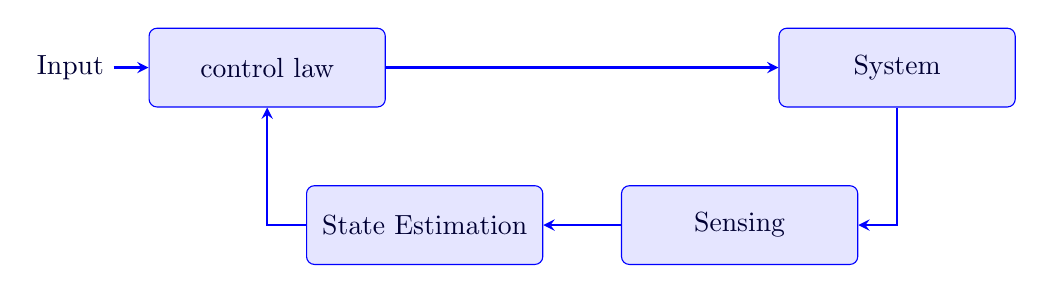
\begin{tikzpicture}[node distance=2cm]
        \node (in) [eNode] {Input};
        \node (control) [recNodeB, right of=in, xshift=0.5cm] {control law};
        \node (sys) [recNodeB, right of=control, xshift=6cm] {System};
        \node (sensor) [recNodeB, below of=sys, xshift=-2cm] {Sensing};
        \node (estimator) [recNodeB, below of=control, xshift=2cm] {State Estimation};
        
        \draw [arrowB] (in) -- (control);
        \draw [arrowB] (control) -- (sys);
        \draw [arrowB] (sys) |- (sensor);
        \draw [arrowB] (sensor) -- (estimator);
        \draw [arrowB] (estimator) -| (control);
    \end{tikzpicture}
    
    \caption{A typical control loop system.
    \label{fig:control loop}}
\end{figure}


%In this thesis we suggest a novel technique where the control loop is composed (as usual) from control tasks and state estimation tasks. 
%And the requirement of the periodical requirements of the control tasks dynamically change and depend on the level of the environmental noise that is expressed by the accuracy of the state estimation (retrieve from estimation loops) and the stability of the system (retrieve from the control loop).


\section{Case studies}
\label{sec:Case study}

\subsection{Vision based controllers for drones}
To test our concepts, we will examine the implementation of an autonomously flying quad-rotor in the context of an agriculture case study. Specifically, we will implement a quad-rotor that flies in corridors and greenhouses by a vision based feedback. The challenge in this case study, from our perspective, is that image processing is a heavy computational task that requires careful scheduling in order to preserve the system predictability and stability.

%TODO Gera: some bla-bla about the current state of the art and how we will improve it. 

In Section~\ref{sec:Research Plan} we suggest a novel framework model for such systems that we will implement in this thesis.

\subsection{Nano-Satellite}
Another interesting case study we will examine is the control of a nano-satellite, in particular scheduling the sensing tasks of \textit{IAI}\footnote{IAI: Israel Aerospace Industries} nano satellites. Their satellites are controlled by a small and relatively slow processor, and the developers say that the main issue in programing the satellite is how to schedule the sensing tasks.
The common approach they are using is to periodically schedule all the sensing task every iteration, and they say that this is the main computational consumption and is too much for their slow processor.

We think that lots of the sensing are unnecessary and the controlling task can be achieved without "most up-to-date" information, some times we can base on good estimation of the sensing value or even use the last value. Although Vision based drones is our main case study, we will also check the possibility to improve the nano-satellite issue with our framework.

\section{Research Plan}
\label{sec:Research Plan}

Our research plan consists of: (1) Designing a methodology for effective allocation of computational resources in real-time control systems; and then (2) Demonstrating our methodology with a framework for developing such systems and with a case study. The details of these two steps are elaborated below.


\begin{figure}[]
    \centering
    
    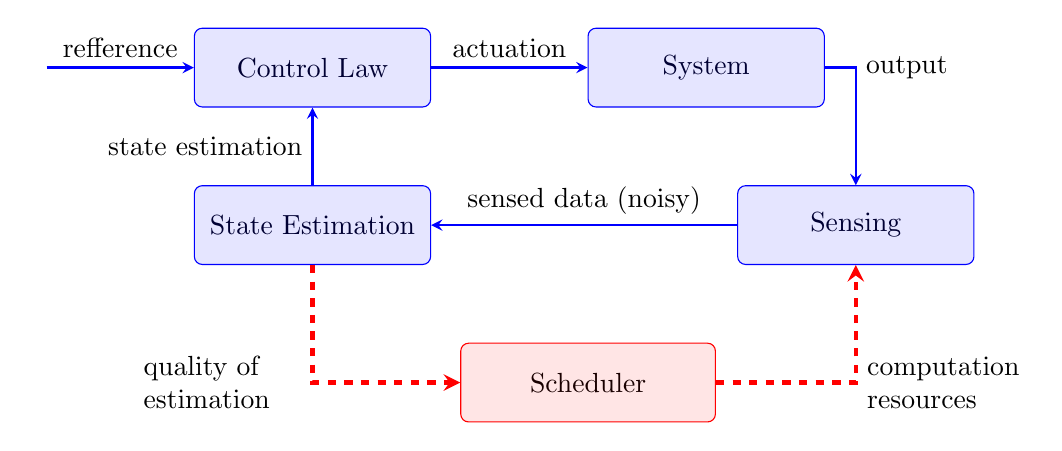
\begin{tikzpicture}[node distance=2cm]
        \node (in) [eNode] {};
        \node (control) [recNodeB, right of=in, xshift=1.5cm] {Control Law};
        \node (sys) [recNodeB, right of=control, xshift=3cm] {System};
        \node (sensor) [recNodeB, below of=sys, xshift=1.9cm] {Sensing};
        \node (estimator) [recNodeB, below of=control] {State Estimation};
        \node (sched) [recNodeG, below of=estimator, xshift=3.5cm, text width=3cm] {Scheduler};
        
        \draw [arrowB] (in) -- node[above] {refference} (control);
        \draw [arrowB] (control) -- node[above] {actuation} (sys);
        \draw [arrowB] (sys) -| node[right] {output} (sensor);
        \draw [arrowB] (sensor) -- node[above] {sensed data (noisy)} (estimator);
        \draw [arrowB] (estimator) -- node[left] {state estimation} (control);
        
        \draw [arrowG] (sched) -| node[right,text width=2cm] {computation resources} (sensor);
        %\draw [arrowG] (sched) --  node[right] {$cov(v)$} (estimator);
        \draw [arrowG] (estimator) |- node[left,text width=2cm] {quality of estimation} (sched);
        
        
    \end{tikzpicture}
    
    \caption{Our proposal of a general controller framework. Each control loop (depicted in blue) informs the resource allocator (Scheduler) of its quality of estimation and the allocator allocates accordingly the computation resources among all the control loops. The noise in the sensed data is a function of the amount of computation resources. The more resources are invested in sensing the better (less noisy) sensed data is obtained.
    \label{fig:general_hybrid_loop}}
\end{figure}

\begin{figure}[h]
    \centering
    %TODO - maybe add \%CPU arrow from scheduler to control law 
    %TODO - replace with tikzpicture
    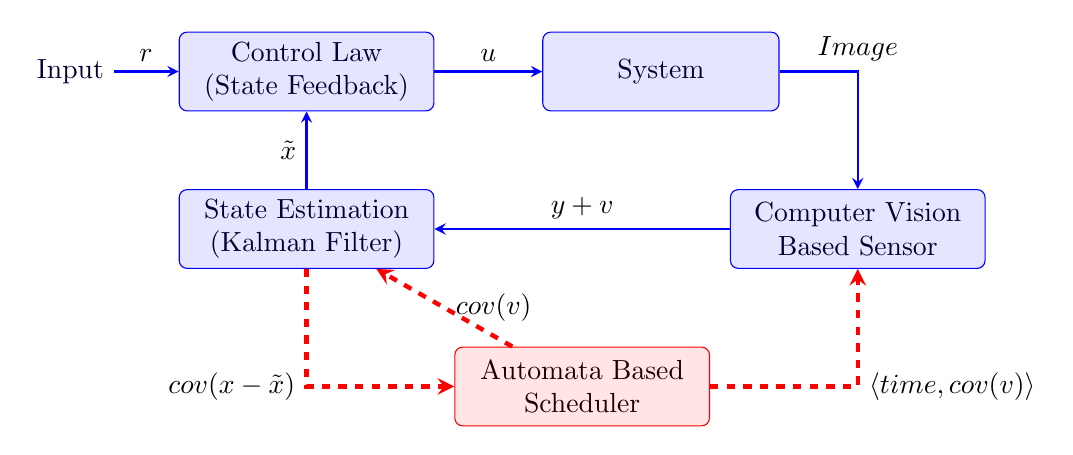
\begin{tikzpicture}[node distance=2cm]
        \node (in) [eNode] {Input};
        \node (control) [recNodeB, right of=in, xshift=1cm, text width=3cm] 
            {Control Law (State Feedback)};
        \node (sys) [recNodeB, right of=control, xshift=2.5cm] {System};
        \node (sensor) [recNodeB, below of=sys, xshift=2.5cm, text width=3cm] 
            {Computer Vision Based Sensor};
        \node (estimator) [recNodeB, below of=control, text width=3cm] 
            {State Estimation (Kalman Filter)};
        \node (sched) [recNodeG, below of=estimator, xshift=3.5cm, text width=3cm] {Automata Based Scheduler};
        
        \draw [arrowB] (in) -- node[above] {$r$} (control);
        \draw [arrowB] (control) -- node[above] {$u$} (sys);
        \draw [arrowB] (sys) -| node[above] {$Image$} (sensor);
        \draw [arrowB] (sensor) -- node[above] {$y+v$} (estimator);
        \draw [arrowB] (estimator) -- node[left] {$\tilde{x}$} (control);
        
        \draw [arrowG] (sched) -| node[right] {$\langle time,cov(v) \rangle$} (sensor);
        \draw [arrowG] (sched) --  node[right] {$cov(v)$} (estimator);
        \draw [arrowG] (estimator) |- node[left] {$cov(x-\tilde{x})$} (sched);
        
    \end{tikzpicture}
    
    \caption{The controller framework we will implement, the $scheduler$ will allocate CPU time ($<time,cov>$) for the  $Computer Vision$ task base on the state estimation certainty using guarded Automata.
    \label{fig:hybrid loop}}
\end{figure}

\subsection{The proposed methodology}
\label{sec:our proposal}

The general methodology that we will develop is illustrated in Figure~\ref{fig:general_hybrid_loop}.
The methodology comes to support an efficient scheduling protocols in modern control systems consisting of a computer that runs many tasks that implement the control laws of independent control loops. 
The current state of art is that the designers of each control loop specify a fixed rate for invocations of the corresponding control task.
%That methodology is based on modern controller architecture where the system has multiple controlling tasks (control loops) and a scheduler that schedule the task as they demand.
% TODO: Use the terminology of the figure
In our methodology, shown in Figure~\ref{fig:general_hybrid_loop}, there is a strong relation between the $Scheduler$ and the control loops. We suggest that each control loop (blue components) will tell the resource allocator ($scheduler$) its level of certainty and the allocator will allocate the CPU time among all the control loops corresponding to the loops certainty in order to maintain some pre-defined specifications of state certainty or stability.

Our proposal is general and may be applicable in a wide range of applications. However, in this initial phase of the research, we believe that it is better to focus on a specific sub-domain and solve all technical issues in order to prove the concept.
In this thesis we will develop and implement the framework shown in Figure~\ref{fig:hybrid loop}: a vision based controller for drone. 

% TODO: Use $ only for math. furmulas
As shown in Figure~\ref{fig:hybrid loop}, the suggested control system framework have strong relation between the tasks scheduler to the control loops, in this case the estimation task ($State~Estimation$) accuracy strongly depends on the sensing task ($Computer~Vision$) and there both collaborate with the $scheduler$ in order to achieve they \textbf{control objectives} (g.e. stability).
In this framework the scheduler is part of the control logic and therefore it can make scheduling decisions based on the current control state, the scheduling of $Computer~Vision$ task is depends on the accuracy of state estimation.
For example if the vision is clear the $Computer~Vision$ will produce good measurement of the $System$ and therefore good accuracy will be achieved so the $Scheduler$ can allocate less computation time to the heavy $Computer~Vision$ task and still remain stable and allocate more CPU to others control loops or some background tasks (like navigation).

The above collaboration requires to re-adjust some parts of the controlling system, e.g. the $State~Estimator$ needs to work with variable error covariance of $Computer~Vision$ measurement and the $Computer~Vision$ needs to be able run within variable time limits, and also the tasks pre-defined requirements need to be re-adjust in order to define the relation between tasks, like $Computer~Vision$ and $State~Estimator$.
Below we will dive in each part of the above system (Figure~
ef{fig:hybrid loop}) and explain how it will be adjusted (changed) and how we will achieve that adjustment in our demonstration.

Finally, we need to re-consider the system Analyzing technique because variable sensing characteristics ($Computer~Vision$ time limits) will lead to variable estimation characteristics... %TODO - complete and fix this paragraph or remove it

\subsubsection{Sensors ($Computer~Vision~Based~Sensor$)}
\label{sec:sensors}
%Anitime reserch of zilbershtain (\cite{Shlomo})
%contract based
%http://ardupilot.org/copter/docs/common-mouse-based-optical-flow-sensor-adns3080.html

$Computer~Vision~Based~Sensor$ is the module that is responsible for taking picture or series of pictures and for producing measurements of quantities such as speed and position relative to the environment.
In our research we will use the $Computer~Vision$ in order to detect two dimensional movement in the camera surface (i.e. the drone speed).
There are many such algorithms (optical flow), they differ by their running time and by the accuracy of the solution, mostly more time lead to more accuracy.

In our case we need to be able to control the $Computer~Vision$ running time and to have some good knowledge of the solution accuracy in order to achieve optimal state estimation (see Section~\ref{sec:estimator}).
We assume that the $Computer~Vision$ error is spread normally, and we will use the error covariance as the solution accuracy. 
We believe that this is a reasonable  assumption because it is the sum of many independent random variables, as follows. Optic flow algorithms usually go by identifying similar regions in consecutive pictures and then averaging the distances that each feature ``traveled''. Assuming that the error in measurement of each feature is independent of the other errors, we get that the total error is the average of independent random variables. We will validate this assumption by experimentation with different parameters of different algorithms.

%TODO - reed a litle the article (\cite{UPenn-Pant}) and re-write the next.
%TODO - check if Anitime reserch (\cite{Shlomo}) can fit here.
%TODO - Make sure that we use the terms contract-base and any-time correctly
In order to control the running time, we will use a "contract based" vision algorithms proposed by Pant~\cite{UPenn-Pant}.
This type of algorithms run until we stop them, and when we stop them they will provide a solution with accuracy that is proportional to the amount of time it was running. That way we can control the solution accuracy by controlling the running time.
In our implementation, in order to lower the complexity, we will pre-define few different ``operation modes" of the $Computer~Vision$ task, that differ by their running time and they are identified by a pair $\langle RunTime, Covariance \rangle$ where $Covariance$ is the error covariance of running time $RunTime$.

\subsubsection{State Estimator}
\label{sec:estimator}
% kalman filter & ...
% seperation rule of kalman
%TODO - complete

\subsubsection{Control Tasks}
% TODO: LQR instead (or in addition?) of PID
The control task itself ($Control Law$) is responsible for reducing the difference between the current state ($x$) where $\tilde{x} = x+ ``estimation~error"$ (in Figure~\ref{fig:general_hybrid_loop}) and the target state ($u$ in Figure~\ref{fig:general_hybrid_loop}), by changing the drone motors speed.
This task is usually a very low CPU consumer and been well studied~\cite{PID}, hence, in this thesis we will use a well known technique from control theory called {\textbf{PID}\footnote{PID controller - A proportional-integral-derivative controller}}. 
In this technique the control output is based on the physical knowledge of the system dynamics, and have 3 variable parameters (P, I and D) that define the controller convergence behavior. 
This is also the technique used in the APM software (Section~
ef{sec:APM}) that we will use and we will not change it.
%TODO - maybe add explanation on how this task can be envolved in the scheduling desision

\subsubsection{Automata Based Scheduler}

%This research continues/completes the work of Merav Bukra ~\cite{Merav} on scheduling computations in embedded control systems.
%In her thesis Merav presented an approach and a proof-of-concept tool for scheduling computation resources in control software. The tool was good enough for demonstrating the concept with simulations, but it did not integrate with any real-life system. In this research we will develop a resource scheduler for real-life control model (see~\ref{sec:contmode}),and upgrade the control software (APM) of a well-known quad-copter by replacing it's RT-scheduler with our new scheduler.
%We expect an improvement in CPU utilization that will allow improvements of stability of the drone.

\subsection{Experimental environment}
\subsubsection{Drones}
\subsubsection{Ardu-Pilot-Mega as base controller software}
\label{sec:APM}

\section{Preliminary Results}
Blablabla said Nobody ~\cite{Merav}.
Blablabla said Nobody ~\cite{APM}.
Blablabla said Nobody ~\cite{RTComposer}.



%\begin{samepage}
    \bibliographystyle{plain}
    \bibliography{proposal}{}
%\end{samepage}

\end{document}}